\documentclass[mathserif]{beamer}
\usepackage{amsmath}
\usepackage{url}
\usepackage{tikz}
\beamertemplatenavigationsymbolsempty
\mode<presentation>
\usetheme{Madrid}
\AtBeginSection[]{}
\setbeamerfont{footnote}{size=\tiny}
\title{Phase Transitions and Scale Free Phenomena in Networks of Memristive Elements}
\author{Forrest Sheldon}
\institute{UCSD}
\date{August 7, 2015}
\titlegraphic{
\includegraphics[width=2.5cm]{gl-1-logo.png}}
\begin{document}

\begin{frame}
\titlepage
\end{frame}

\begin{frame}
\frametitle{A Perspective On Memristors}
\setbeamercovered{static}
\begin{columns}
\column{0.5\textwidth}
\begin{center}
\onslide<1->{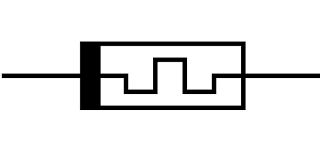
\includegraphics[width=0.17\textwidth]{memristor.png}}

\only<1>{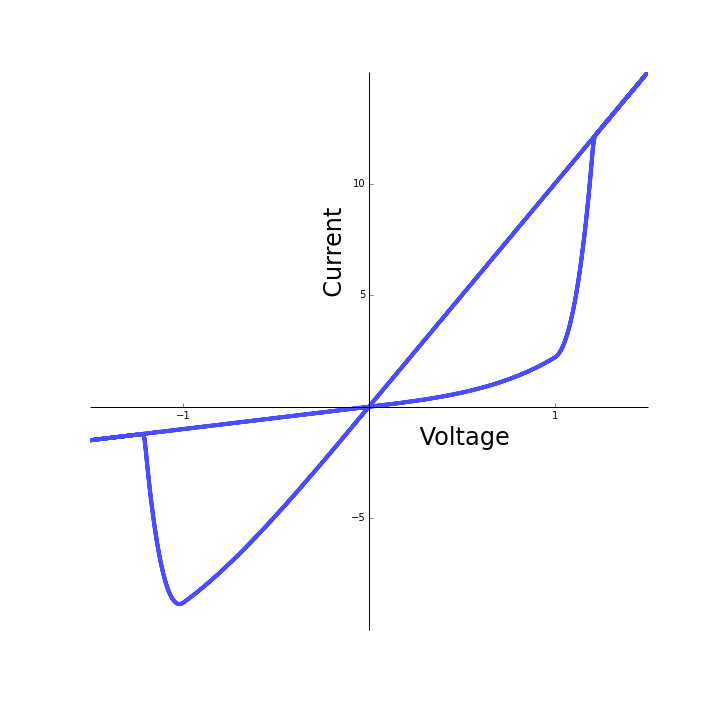
\includegraphics[width=0.65\textwidth]{hysteresis.png}}

\only<2>{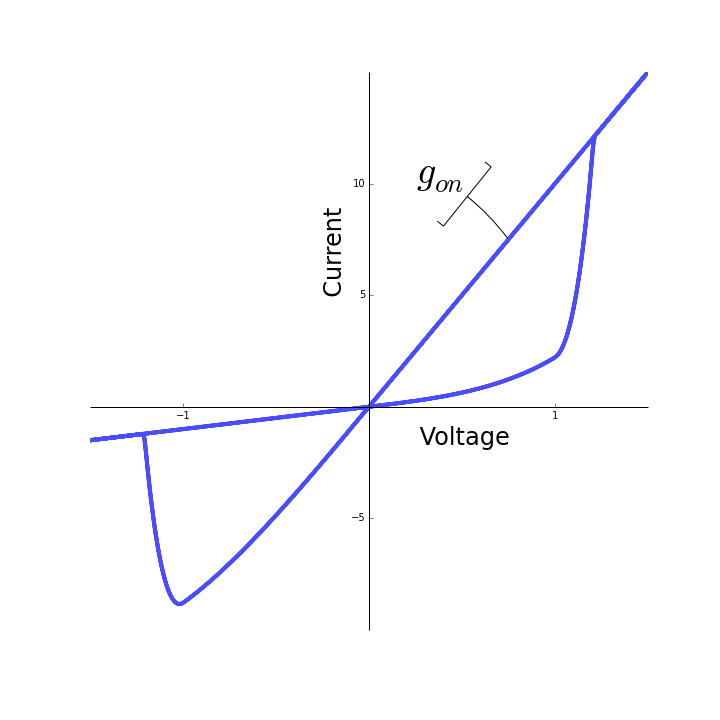
\includegraphics[width=0.65\textwidth]{hysteresis_on.png}}

\only<3>{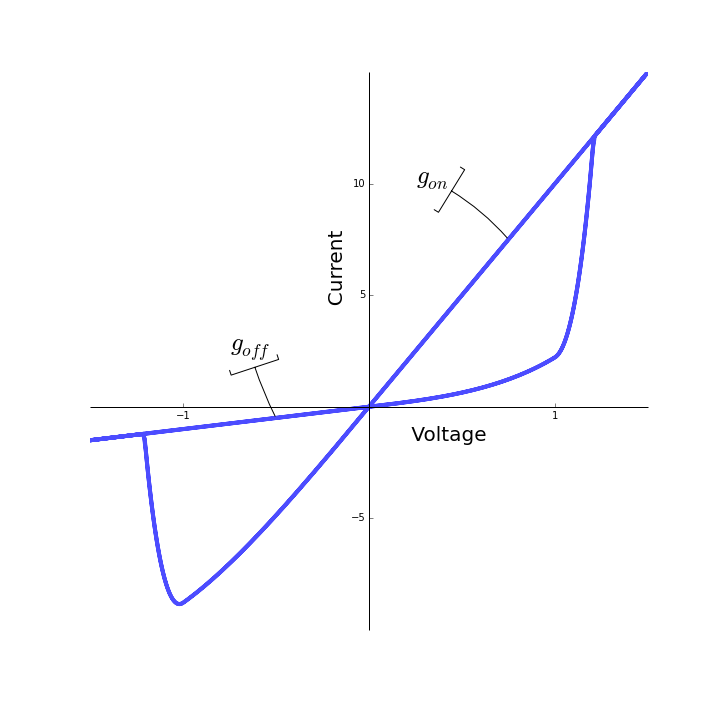
\includegraphics[width=0.65\textwidth]{hysteresis_off.png}}

\onslide<4->{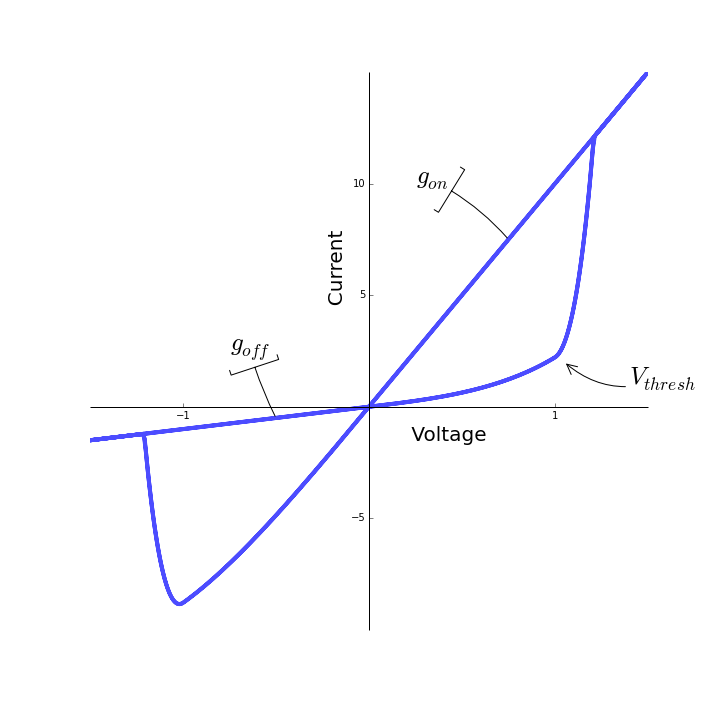
\includegraphics[width=0.65\textwidth]{hysteresis_thresh.png}}
\end{center}
\column{0.5\textwidth}
\centering
\onslide<6->{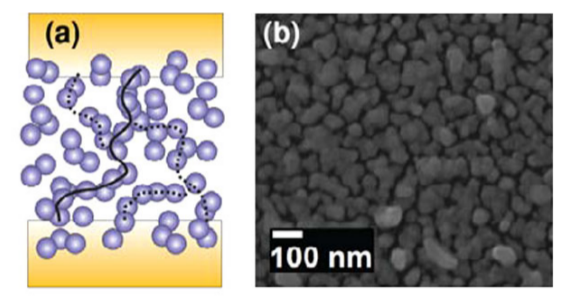
\includegraphics[width=0.65\textwidth]{Granular_short.png}}
\onslide<6->{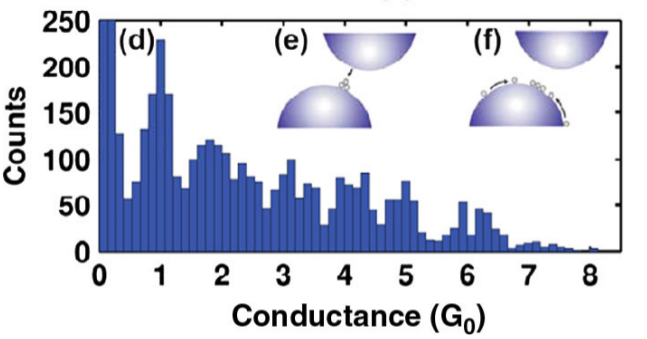
\includegraphics[width=0.65\textwidth]{Granular_low.png}\footnote[frame]{A. Sattar, S.Fostner, and S. Brown, Phys. Rev. Lett. \textbf{111}, 13 (2013).}}
\end{columns}
\begin{center}
\onslide<5->{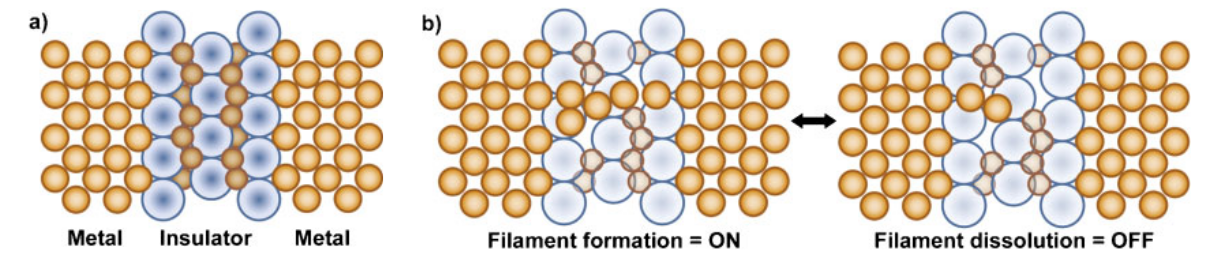
\includegraphics[width=0.8\textwidth]{Atomic_Switch_Filament.png}\footnote[frame]{A. Z. Steig \emph{et al.}, Jpn. J. Appl. Phys. \textbf{53} 01AA02 (2014).}}

\end{center}

\end{frame}

\begin{frame}
\frametitle{'Nonideal' Properties are Interesting}

\begin{center}
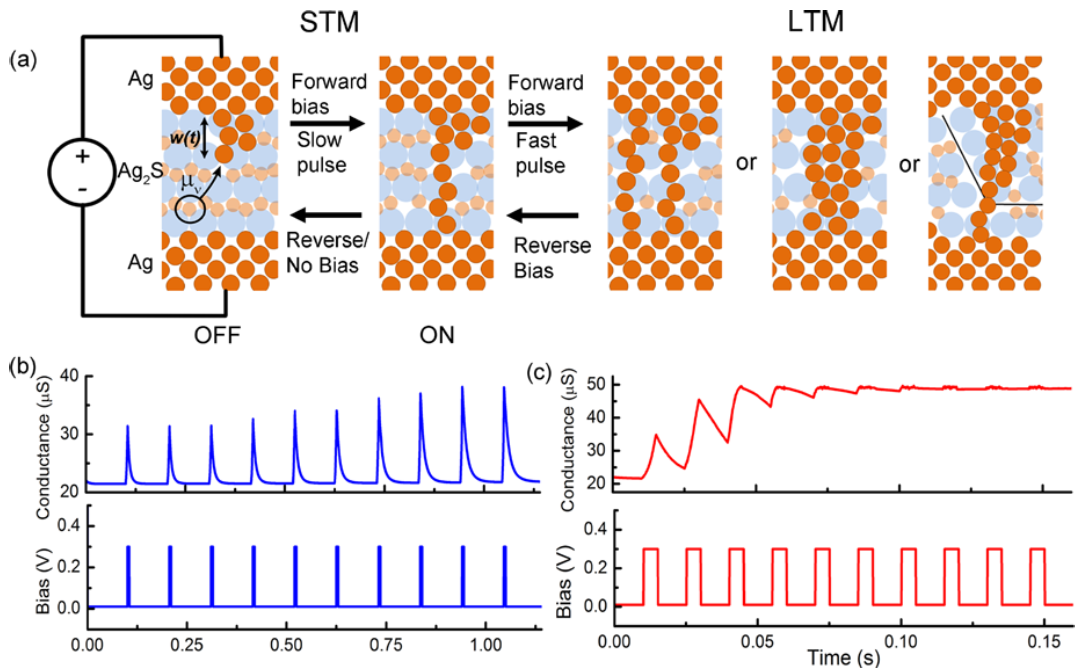
\includegraphics[width=0.8\textwidth]{STM_LTP.png}\footnote{A.Z. Steig \emph{et al.}, in \emph{Memristor Networks}, editted by A. Adamatzky, L. Chua, (Springer International Publishing, 2014)}
\end{center}
\end{frame}

\begin{frame}
\frametitle{Memristive Networks}
\begin{columns}

\column{0.5\textwidth}
\begin{center}
\onslide<1->{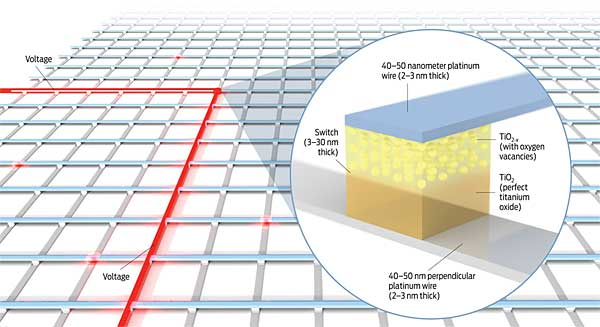
\includegraphics[width=0.7\textwidth]{Crossbar.jpeg}\footnote[frame]{\url{http://spectrum.ieee.org/semiconductors/processors/how-we-found-the-missing-memristor/memrf1}}}
\vspace{0.25in}

\onslide<2->{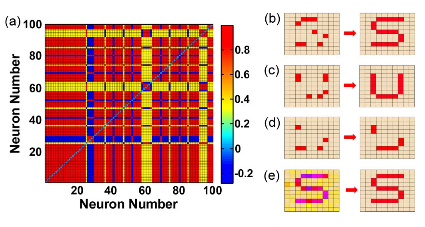
\includegraphics[width=0.7\textwidth]{Associative_Memory.png}\footnote[frame]{D. Kuzum \emph{et al.} IEEE Trans. on Elec. Dev., \textbf{59}, 12 (2012)}}

\end{center}
\column{0.5\textwidth}
\begin{center}
\onslide<3->{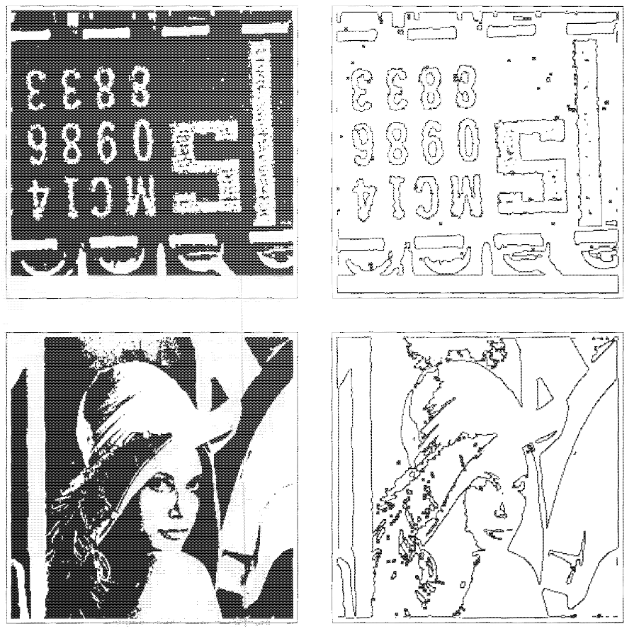
\includegraphics[width=0.5\textwidth]{Cell_Auto_Edge.png}\footnote[frame]{M. Itoh, L. O. Chua, Int.. J. Bifurcat. Chaos, \textbf{19}, 11 (2009).}}
\vspace{0.25in}

\onslide<4->{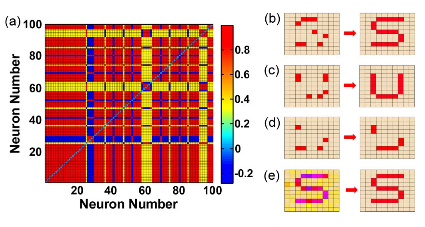
\includegraphics[width=0.7\textwidth]{Associative_Memory.png}\footnote[frame]{CITE}}
\end{center}
\end{columns}
\end{frame}

\begin{frame}
\frametitle{Atomic Switch Network}

\begin{center}
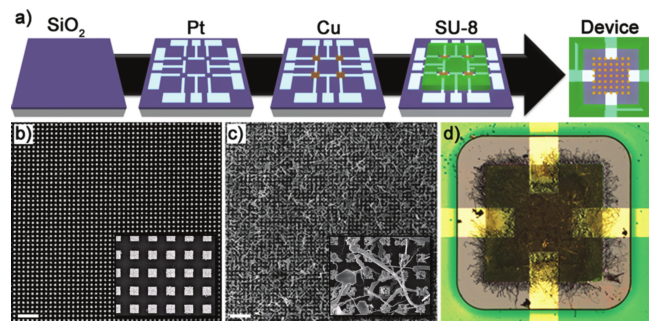
\includegraphics[width=9cm]{ASN_fabrication.png}\footnote{A. Z. Stieg \emph{et al.}, Adv. Mater. \textbf{24}, (2012).}
\end{center}

\begin{columns}
\column{0.5\textwidth}
\centering
\onslide<2->{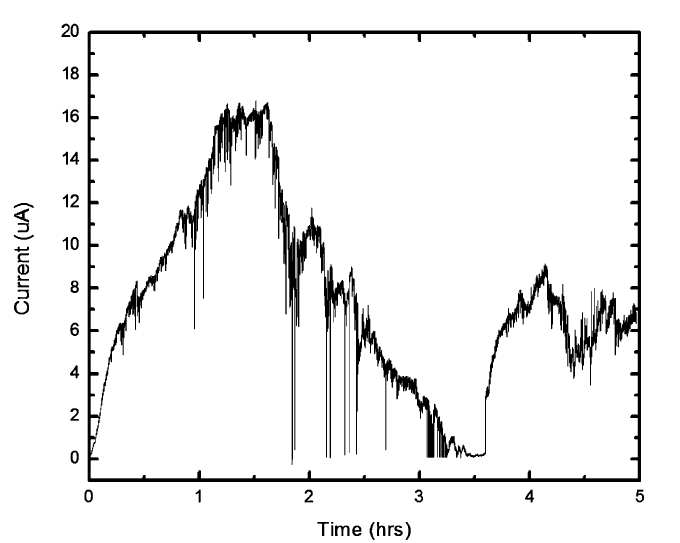
\includegraphics[width=0.5\textwidth]{ASN_fluctuations.png}}
\column{0.5\textwidth}
\centering
\onslide<3->{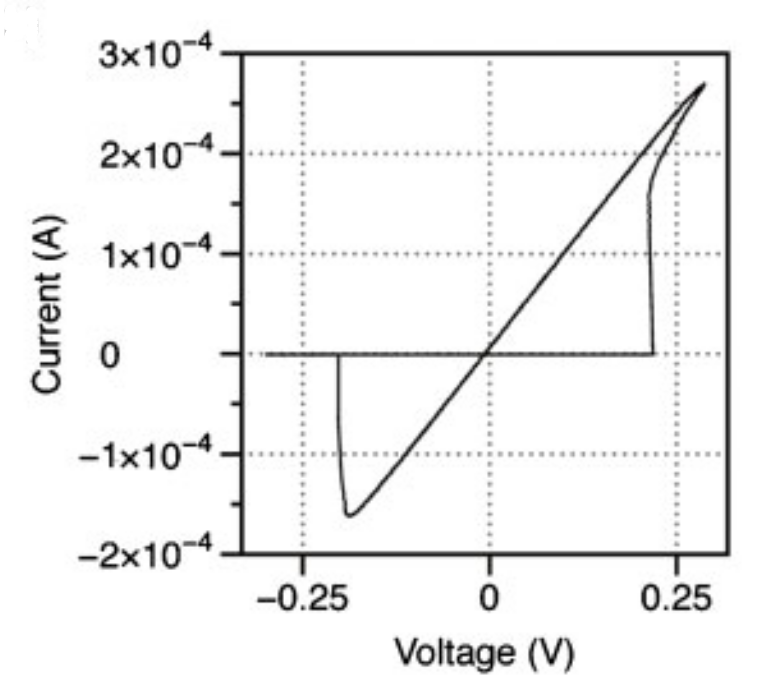
\includegraphics[width=0.5\textwidth]{ASN_hysteresis.png}}
\end{columns}

\end{frame}

\begin{frame}
\frametitle{Questions}
\setbeamercovered{dynamic}
\begin{itemize}
\item<1> Phase Transitions?
\item<2> Role of ON/OFF ratio and disorder?
\item<3> Avalanches?
\end{itemize}
\end{frame}

\begin{frame}
\frametitle{Modeling the Network}
\begin{picture}(320, 250)
\onslide<1->{\put(0, 210){Timescales}}
\onslide<1->{\put(110, 174){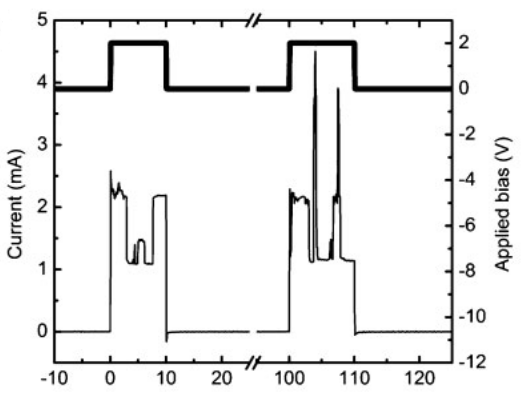
\includegraphics[width=1.25in]{ASN_jumps.png}}}
\onslide<2->{\put(220, 164){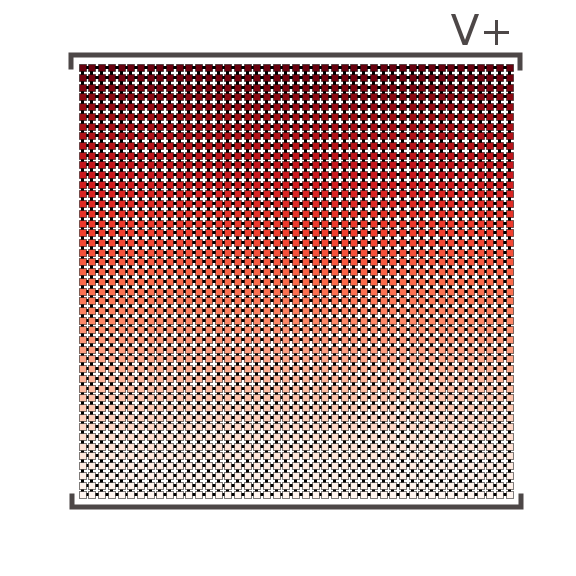
\includegraphics[width=1.2in]{harmonic_voltage_brackets.png}}}

\onslide<3->{\put(0, 160){Thresholds}}

\onslide<4->{\put(0, 110){Network Structure}}
\onslide<4->{\put(120, 103){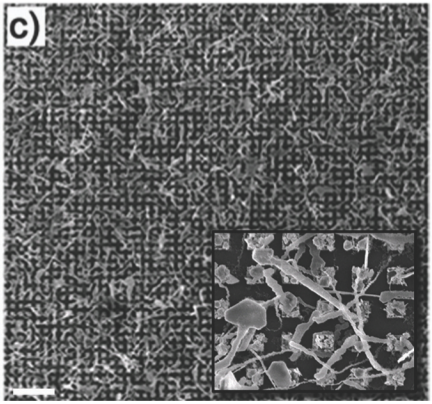
\includegraphics[width=0.95in]{ASN_structure.png}}}
\onslide<5->{\put(220, 91){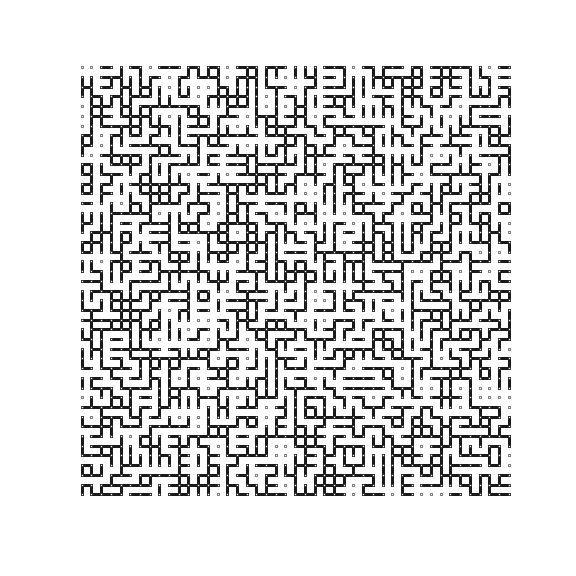
\includegraphics[width=1.2in]{RR_cond.png}}}

\onslide<6->{\put(0, 60){Disordered$\to$Regular}}
\onslide<6->{\put(110, 13){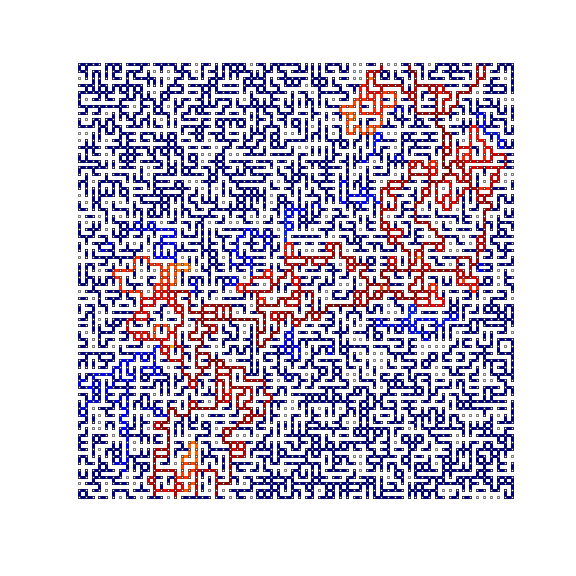
\includegraphics[width=1.2in]{RR_logvoltage.png}}}
\onslide<7->{\put(217, 10){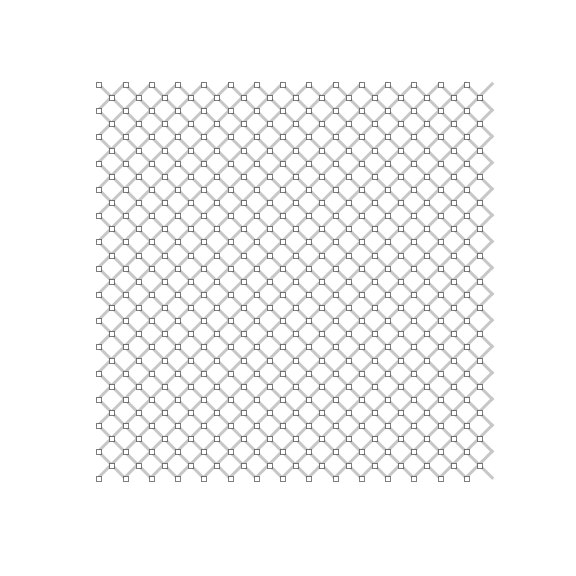
\includegraphics[width=1.3in]{diag_network.png}}}

\end{picture}
\end{frame}

\begin{frame}
\frametitle{Our Model}
\begin{columns}
\column{0.5\textwidth}
\begin{center}
\onslide<1->{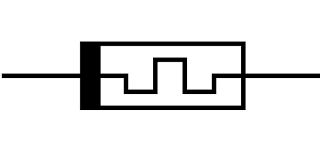
\includegraphics[width=0.25\textwidth]{memristor.png}}

\only<1>{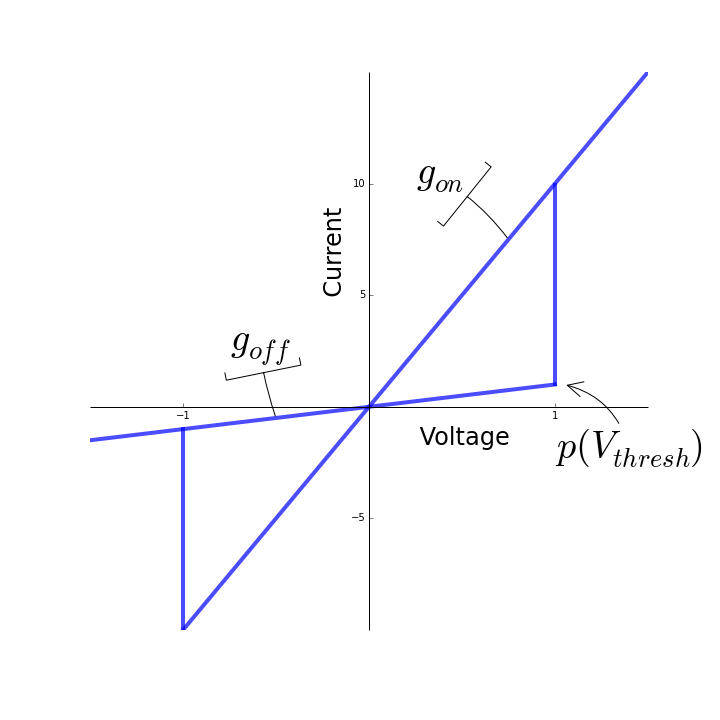
\includegraphics[width=\textwidth]{memristor_model.png}}
\onslide<2->{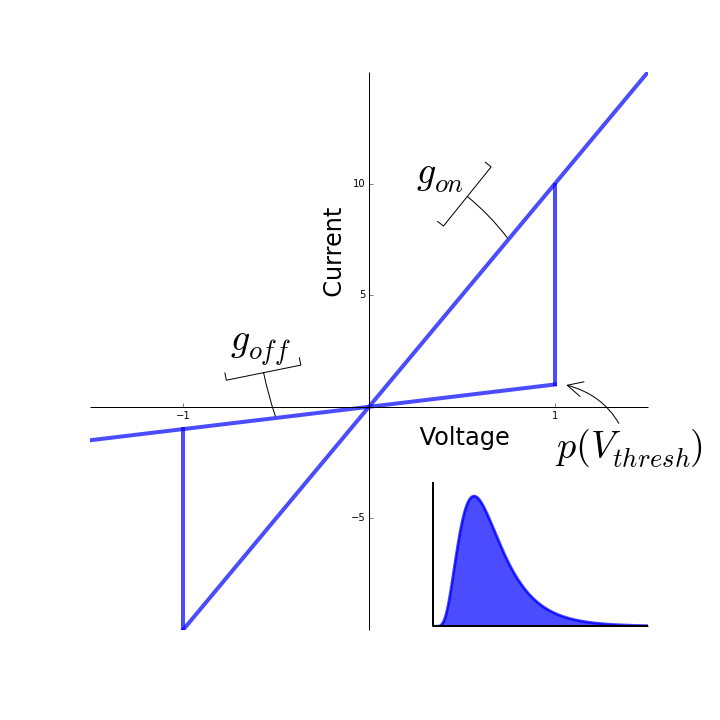
\includegraphics[width=\textwidth]{memristor_model_dist.png}}
\end{center}
\column{0.5\textwidth}
\centering
\onslide<3->{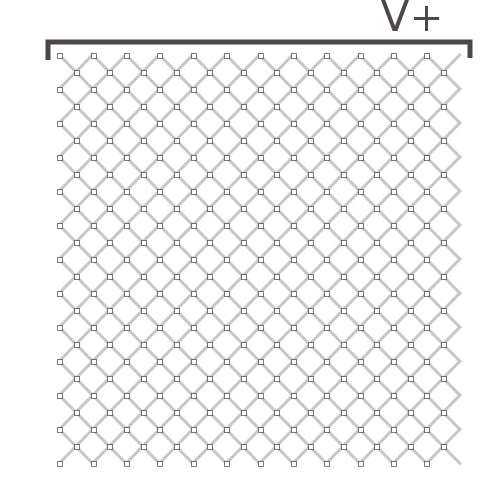
\includegraphics[width=0.4\textwidth]{Inside_a_network_1.png}}

\onslide<4->{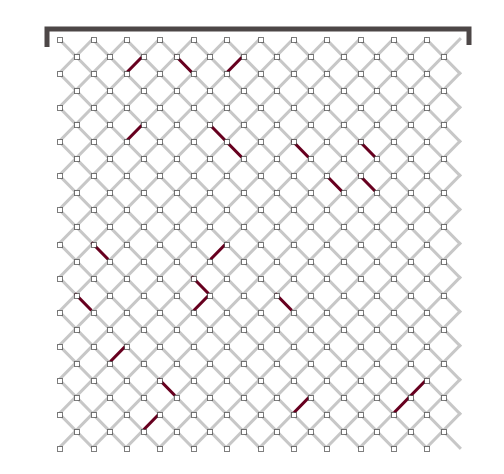
\includegraphics[width=0.4\textwidth]{Inside_a_network_2.png}}

\onslide<5->{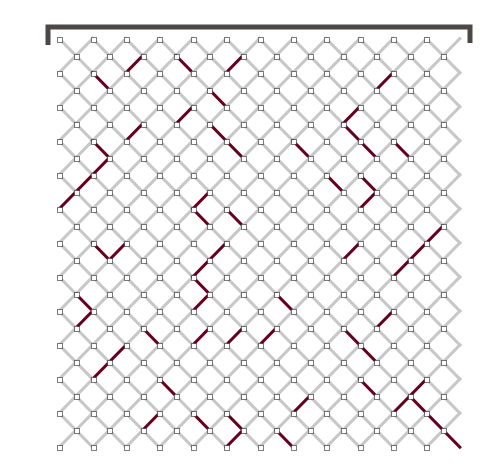
\includegraphics[width=0.4\textwidth]{Inside_a_network_3.png}}

\end{columns}
\end{frame}

\begin{frame}
\frametitle{Simulation Results}
\begin{columns}
\column{0.5\textwidth}
\onslide<1->{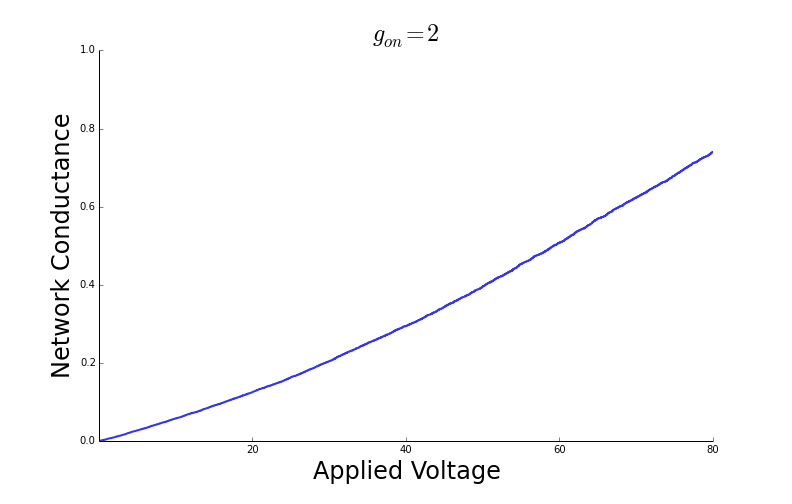
\includegraphics[width=\textwidth]{2DL45ON2_cond.png}}

\onslide<2->{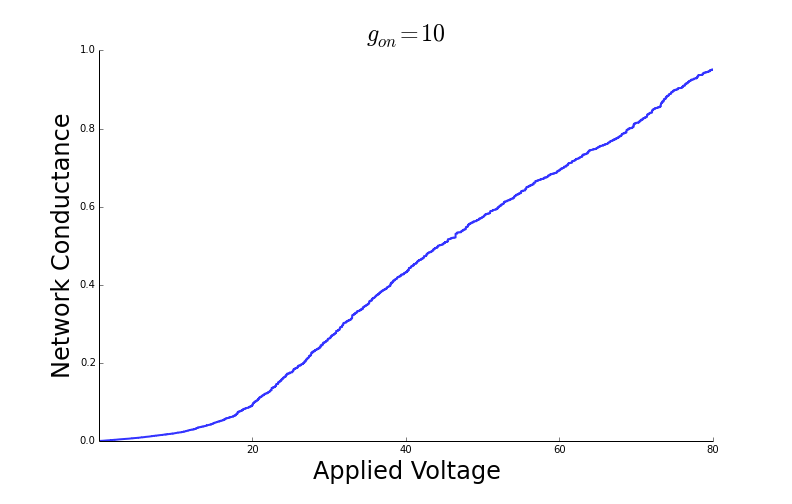
\includegraphics[width=\textwidth]{2DL45ON10_cond.png}}

\column{0.5\textwidth}
\onslide<3->{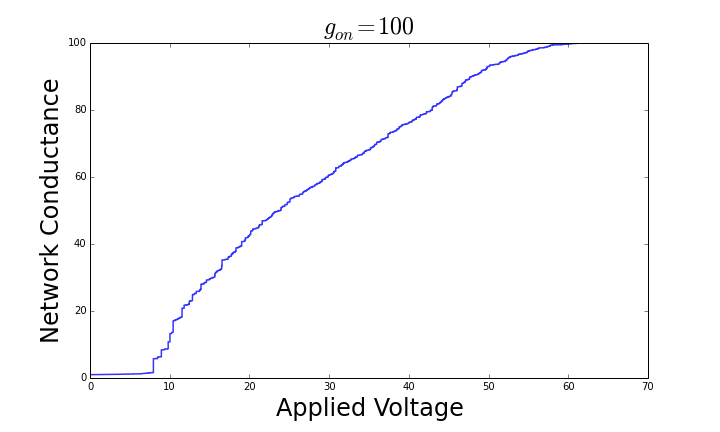
\includegraphics[width=\textwidth]{2DL45ON100_cond.png}}

\onslide<4->{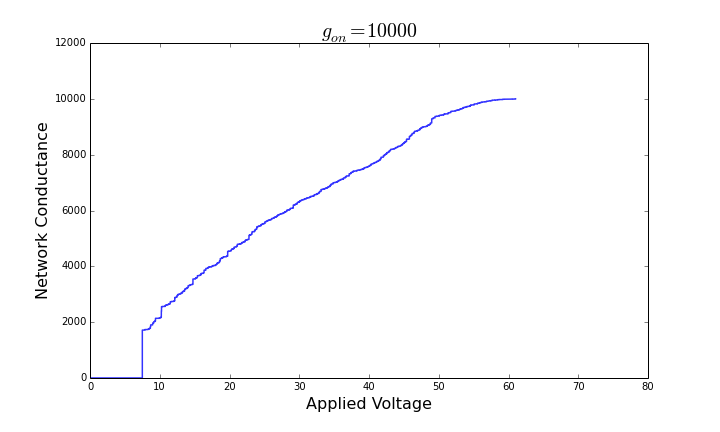
\includegraphics[width=\textwidth]{2DL45ON10000_cond.png}}

\end{columns}
\end{frame}

\begin{frame}
\frametitle{Internal Dynamics}

\end{frame}

\begin{frame}
\frametitle{Mean-Field Theory}

\onslide<1->{$$P = \sum_i \sigma_i \Delta V_i^2$$}

\onslide<2->{$$P = G(\{\sigma_i\})V^2$$}

\onslide<3->{Effective Medium Theory, $G(\{\sigma_i\}) \approx G(f), \quad f = \frac{n_{on}}{N}$}

\onslide<4->{$$\phi = \frac{\sum_i \sigma_i}{N} = \phi(f)\quad G(f) \to G(\phi)$$}

\onslide<5->{$$P = \sum_i \sigma_i \frac{G(\phi)V^2}{\phi N}$$}


\end{frame}

\begin{frame}
\frametitle{Mean-Field Theory}

\onslide<1->{$$\Delta V_{MF} = \sqrt{\frac{G(f)}{\phi(f)}}\frac{V}{\sqrt{N}} = h(f)v$$}
\onslide<2->{Self-Consistency Equation,
$$f = \int_0^{h(f)v} p(t) dt$$

\begin{center}
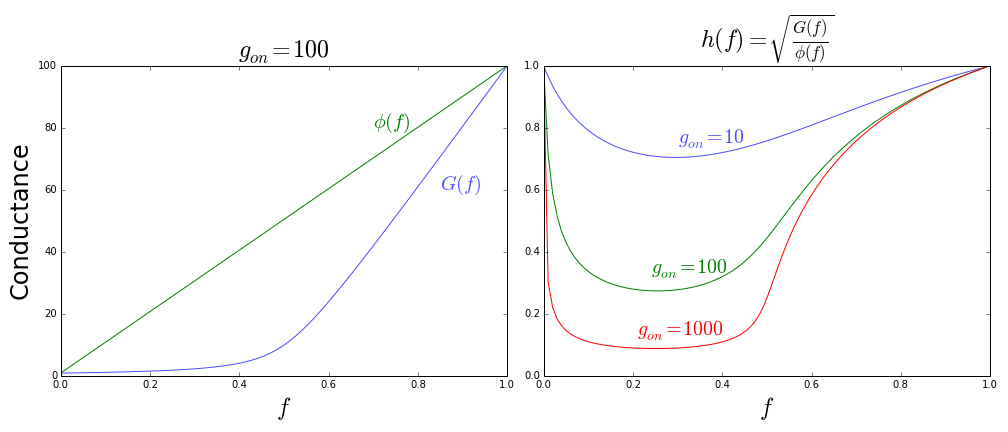
\includegraphics[width=0.8\textwidth]{MF_upper_limit.png}
\end{center}
}
\end{frame}

\begin{frame}
\frametitle{One-Dimensional Networks}
\centering
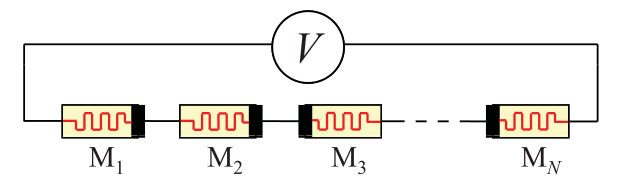
\includegraphics[width=0.4\textwidth]{1D_memristor_chain.png}

\begin{columns}
\column{0.5\textwidth}
$$G(f) = \frac{g_{on}g_{off}}{N(g_{on} - f (g_{on} - g_{off}))}$$
\centering
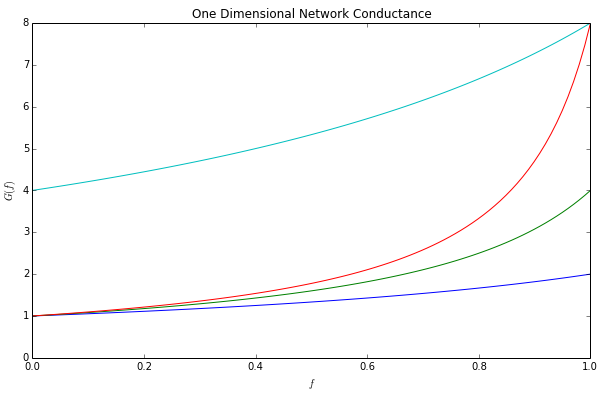
\includegraphics[width=\textwidth]{1D_Network_Cond.png}

\column{0.5\textwidth}
$$f = \int_0^{G(f)V} p(t) dt$$
\begin{center}
\only<1>{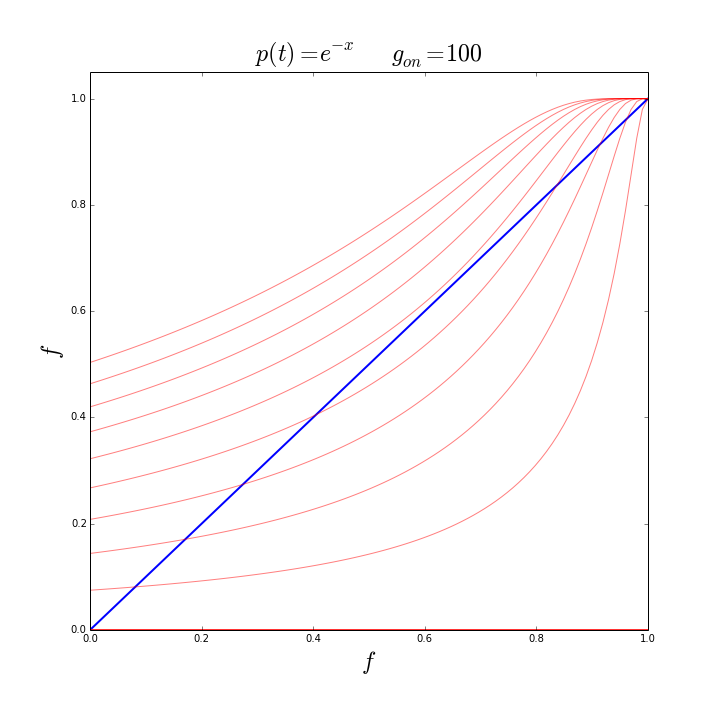
\includegraphics[width=0.8\textwidth]{SC_1D_ON100_expon_0.png}}
\only<2>{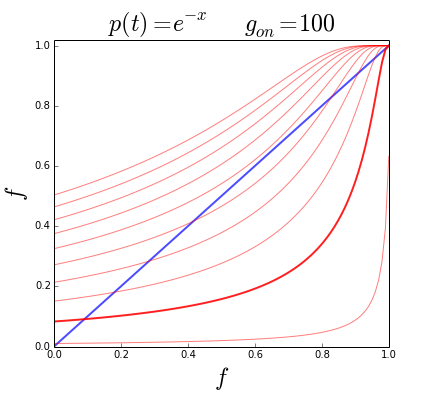
\includegraphics[width=0.8\textwidth]{SC_1D_ON100_expon_1.png}}
\only<3>{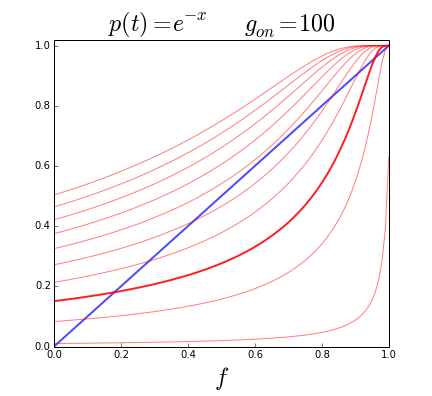
\includegraphics[width=0.8\textwidth]{SC_1D_ON100_expon_2.png}}
\only<4>{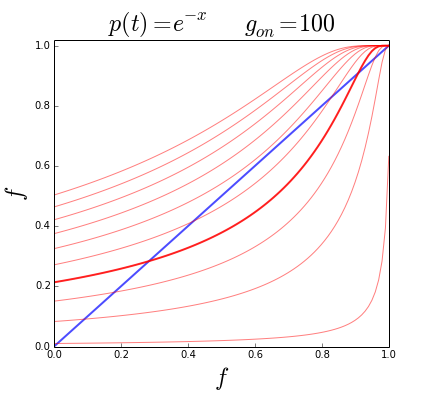
\includegraphics[width=0.8\textwidth]{SC_1D_ON100_expon_3.png}}
\only<5>{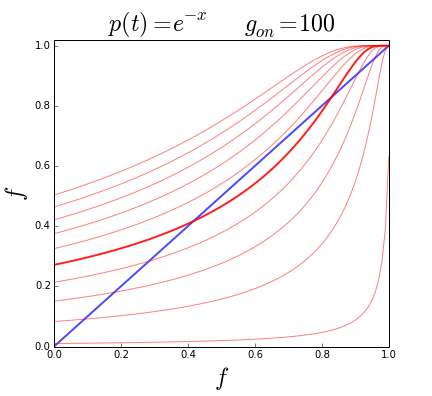
\includegraphics[width=0.8\textwidth]{SC_1D_ON100_expon_4.png}}
\only<6>{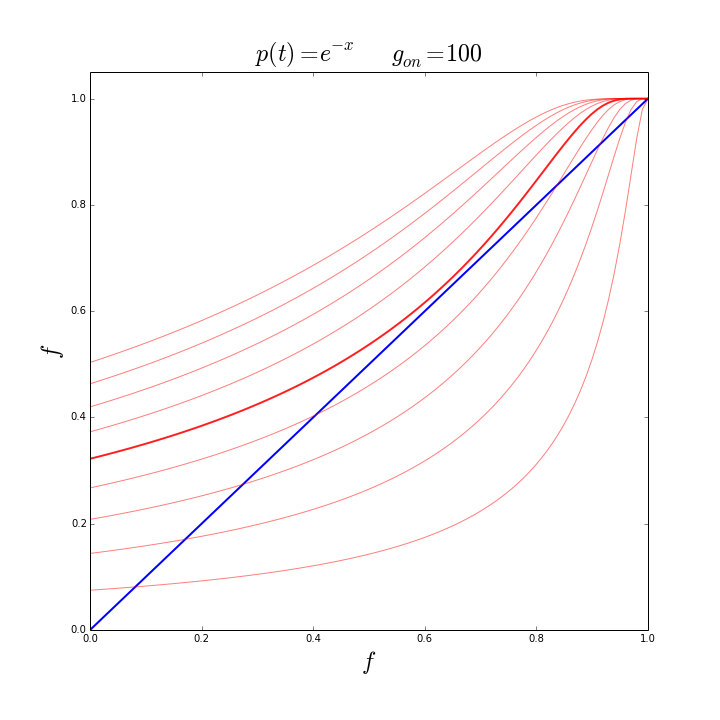
\includegraphics[width=0.8\textwidth]{SC_1D_ON100_expon_5.png}}
\only<7>{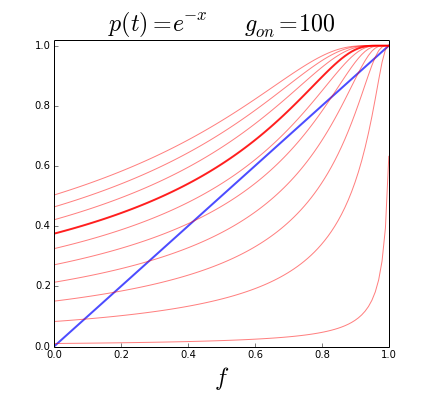
\includegraphics[width=0.8\textwidth]{SC_1D_ON100_expon_6.png}}
\only<8>{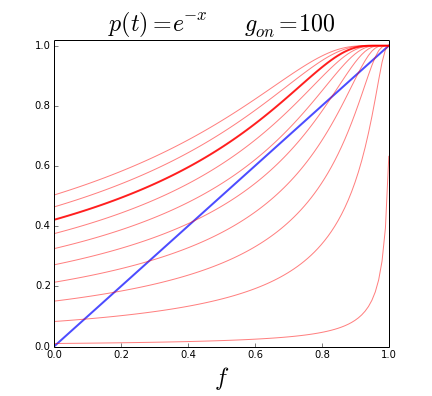
\includegraphics[width=0.8\textwidth]{SC_1D_ON100_expon_7.png}}
\only<9>{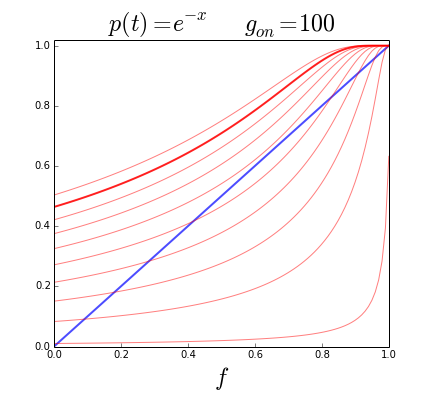
\includegraphics[width=0.8\textwidth]{SC_1D_ON100_expon_8.png}}
\only<10>{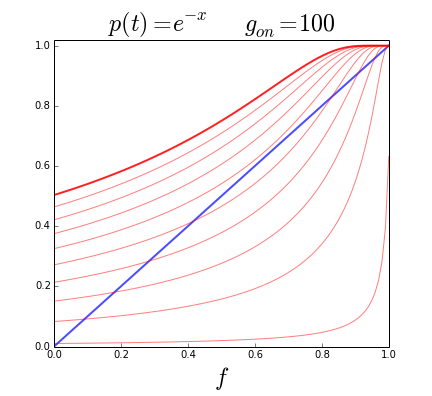
\includegraphics[width=0.8\textwidth]{SC_1D_ON100_expon_9.png}}
\end{center}

\end{columns}
\end{frame}

\begin{frame}
\frametitle{Finding the transition}
First order phase transition:
$$f = \int_0^{G(f)V} p(t) dt,  \quad\quad 1 = p(G(f)V)G'(f)V \quad 0 \le f \le 1$$
For Uniform(0,1),
$f_c = \frac{1}{2(1-\alpha)}, \: V_c = \frac{TN}{4g_{off}(1-\alpha)},
 \: \alpha = \frac{g_{off}}{g_{on}}$
\centering
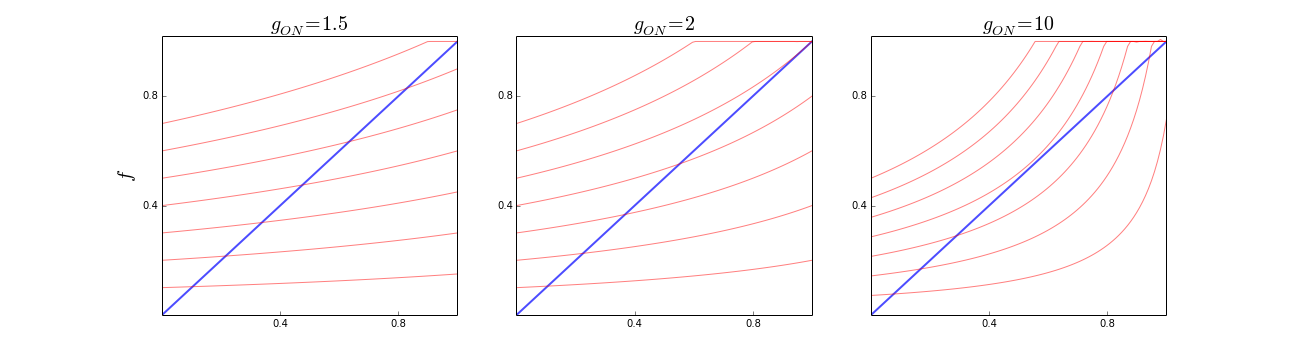
\includegraphics[width=\textwidth]{SC_1D_Uniform01.png}
\end{frame}

\begin{frame}
\frametitle{Finding the Transition}
\centering
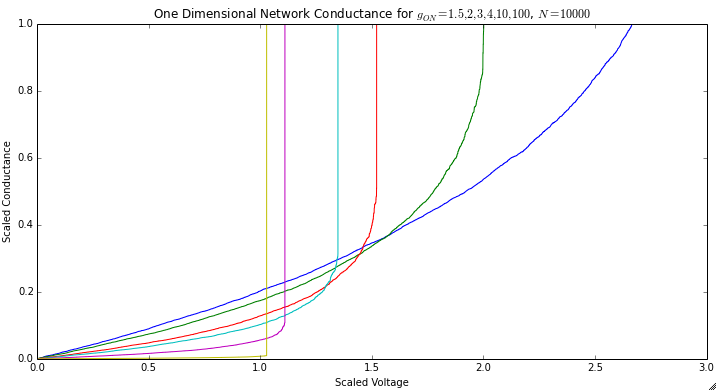
\includegraphics[width=0.8\textwidth]{1D_Cond.png}

\end{frame}

\begin{frame}
\frametitle{Back to 2D}
$p(t) = e^{-t}$
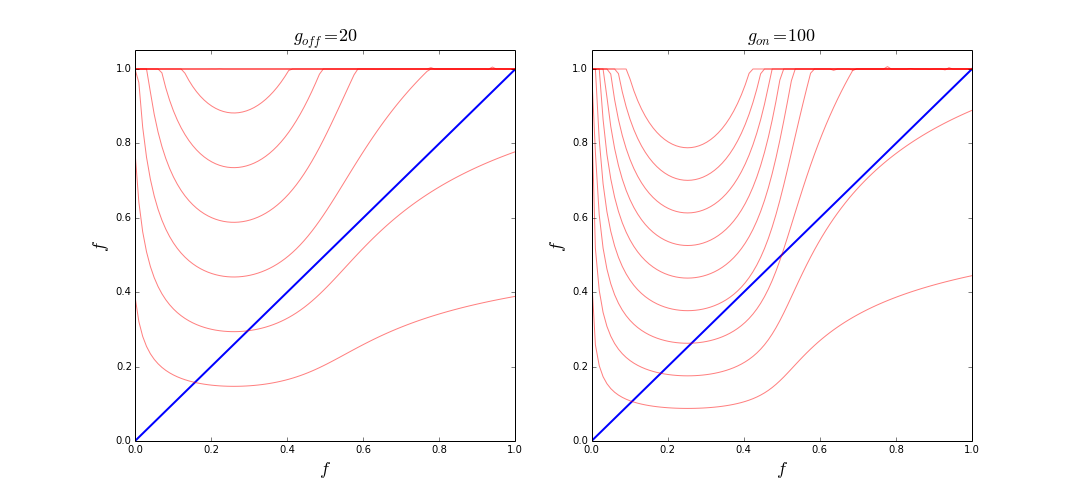
\includegraphics[width=\textwidth]{2D_MF_expon.png}

\end{frame}

\begin{frame}
\frametitle{Avalanches}
\begin{columns}
\column{0.65\textwidth}
\begin{itemize}
\item<2-> Switching a memristor: $f\to f+\frac{1}{N}$

\item<3-> Increases current, $h(f)V\to h(f)V + \frac{h'(f)V}{N}$

\item<4-> $$\frac{\int_{h(f)V}^{h(f)V + \frac{h'(f)V}{N}} p(t) }{\int_{h(f)V}^{\infty} p(t)} \approx \frac{p(h(f)V)h'(f)V}{(1-f)N}$$

\item<5-> $$P(n) \to \frac{(\mu)^n}{n!} e^{-\mu}, \quad \mu = p(h(f)v)h'(f)v$$

\end{itemize}
\column{0.33\textwidth}
\onslide<1->{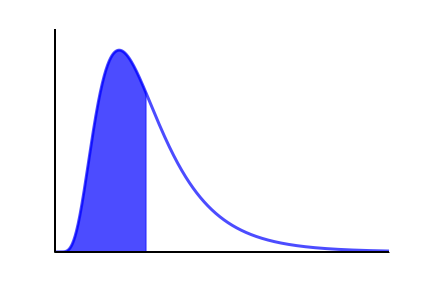
\includegraphics[width=\textwidth]{dist_init.png}}
\onslide<4->{\includegraphics[width=\textwidth]{dist_first_switch.png}}
\onslide<6->{\includegraphics[width=\textwidth]{dist_2nd_switch.png}}
\end{columns}

\end{frame}



\begin{frame}
\frametitle{Branching Process with Poissonian Offspring}




\end{frame}
\begin{frame}
\frametitle{Avalanche Size Distribution}
\begin{itemize}
\item<1-> Branching Process with poissonian offspring distribution
$$P(s) = \frac{(\mu s)^{s-1}}{s!} e^{-\mu(s-1)}$$
\item As $\mu\to 1$ we approach a critical branching process and
$$P(s) \sim s^{-3/2}$$
\end{itemize}
\end{frame}

\begin{frame}
\frametitle{Avalanches in Random Resistor Networks}
\includegraphics[width=0.8\textwidth]{Avalanches_p6.png}

\end{frame}

\begin{frame}
\frametitle{Next Steps}
\begin{columns}
\column{0.5\textwidth}
\begin{itemize}
\item Phase Transitions in Current Controlled Networks
\item Pattern Formation/Structure in Avalanching
\end{itemize}
\column{0.5\textwidth}
\includegraphics[width=\textwidth]{Current_MF.png}

\end{columns}
\end{frame}

\end{document}
